\documentclass[leqno,presentation]{beamer}
\DeclareGraphicsExtensions{.eps,.jpg,.png,.tif}
\usepackage{amssymb, amsmath, pdfpages, amsfonts, calc, times, type1cm, latexsym, xcolor, colortbl, hyperref, bookmark}
\usepackage{graphicx}
\usepackage{tabularx}
\usepackage{multirow}
\graphicspath{ {images/} }

\usepackage[latin1]{inputenc}
\usepackage[english]{babel}
\usetheme{Darmstadt}
\newcommand{\R}{\mathbb{R}}
\newcommand{\N}{\mathbb{N}}
\newcommand{\overbar}[1]{\mkern1.5mu\overline{\mkern-1.5mu#1\mkern-1.5mu}\mkern1.5mu}
\newcommand{\highlight}[1]{
  \addtolength{\fboxrule}{.2ex}
  \begin{block}{}
    \begin{quote}#1
    \end{quote}
  \end{block}
}

\newtheorem*{conjecture}{Conjecture}
\newtheorem*{proposition}{Proposition}

\title{Automatic Theorem Proving}
\author[names]{ Abdullah Dean, Eric Ma, \textbf{Reed Oei}, Tatum Schmidt \\ Christian Schulz (Team Leader) \\ Philipp Hieronymi (Faculty mentor)}

\institute{
  \\[-3ex]
  University of Illinois at Urbana-Champaign
  \\[2ex]
  \includegraphics[width = 0.3\textwidth]{UIUC_logo.png}
  \hspace{.30cm}
  
\includegraphics[width = 0.07\textwidth]{igl-logo-small.png}
  \\[3ex]
  Illinois Geometry Lab  \\ December 4, 2019\\[2ex] }

\date{}

\begin{document}
% Title slide
\frame{\titlepage}

\section{Theorem Proving}

\begin{frame}{Automatic Theorem Proving}
    \begin{itemize}
        \item An \emph{automated theorem prover} is a program that takes a logical statement as input and proves if it is true or false
        
        \item Automated theorem provers have attractive qualities
            \begin{itemize}
                \item Computers are very reliable, and never get tired/bored
                \item Can easily explore new hypotheses
            \end{itemize}
    \end{itemize}
\end{frame}

\begin{frame}{Automata}
    \begin{itemize}
        \item A finite automaton is a ``machine'' that takes as input some finite \emph{word}, e.g., ``abc'', and \emph{accepts} or \emph{rejects} it.
        
        \item A finite automaton can be represented as a \textbf{finite} collection of \emph{states} and \emph{transitions}.
        
        \item The following automata demonstrate the \emph{closure} properites of automata: we can combine automata to express more complicated properties
    \end{itemize}
    
    \begin{figure}[h]
        \begin{minipage}{.3\textwidth}
        \center{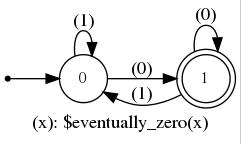
\includegraphics[width=\textwidth]{images/eventually_zero.jpg}}
        \end{minipage}
        \hfill
        \begin{minipage}{.3\textwidth}
        \center{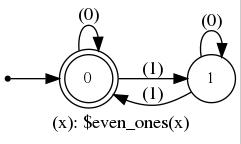
\includegraphics[width=\textwidth]{images/even_ones.jpg}}
        \end{minipage}
        \hfill
        \begin{minipage}{.3\textwidth}
        \center{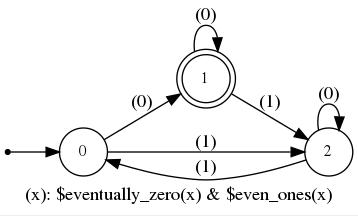
\includegraphics[width=\textwidth]{images/both.jpg}}
        \end{minipage}
    \end{figure}
\end{frame}

\section{Prior Work}

\begin{frame}{Automatic Words}

    \begin{itemize}
        \item An \emph{automatic word} is a sequence such that there is an automaton that outputs the $n$-th character given $n$ in a suitable representation
        \item For example, Sturmian words are automatic words: 
            \begin{itemize}
                \item Imagine hitting a billiard ball at some angle $\theta$
                \item When the ball crosses a vertical line, write a 0; for horizontal lines, write a 1
                \item $C_{1/\phi} = 0100101001\ldots$
            \end{itemize}
    \end{itemize}
    
    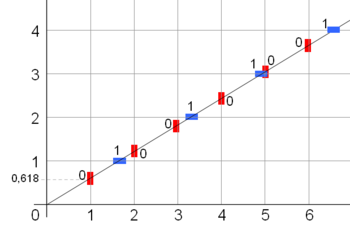
\includegraphics[height=0.4\textheight]{images/Fibonacci_word_cutting_sequence.png}
\end{frame}

\begin{frame}{Prior Results}
    \begin{itemize}
        \item Earlier automated theorem proving efforts on Sturmian words only proved properties of single words
        
        \item Using automata we created and an automated theorem prover (Walnut), we proved the following conjectures, among others, for some infinite classes of Sturmian words:
        
        \begin{conjecture}\label{conj:antisq}
            Every Sturmian word has only finitely many antisquares.
        \end{conjecture}
                    
        \begin{conjecture}\label{conj:grouped}
            Every Sturmian word contains grouped factors.
        \end{conjecture}
        
        \item Limitation: Our current approach cannot prove the above for \textbf{all} Sturmian words
    \end{itemize}
\end{frame}

\section{Progress}

\begin{frame}{Pecan}
\begin{itemize}
    \item We are developing an automated theorem prover that we call Pecan
    \item Pecan uses B\"uchi automata, which take infinite strings as input (c.f., Walnut, which uses finite automata)
    \item We use B\"uchi automata because:
        \begin{itemize}
            \item Some problems are more naturally expressed with B\"uchi automata
            \item Some problems can \textbf{only} be expressed with B\"uchi automata
            \item We can still express properties about finite strings
        \end{itemize}
\end{itemize}
\end{frame}

\section{Future Work}

\begin{frame}{Future Work}
\begin{itemize}
    \item Further develop Pecan into a more effective tool for theorem proving.

    \item Improve on last semester's work on proving statements about \emph{every} Sturmian word using Pecan.
    
    \item Prove properties related to the real numbers, which we can now represent using infinite strings.
\end{itemize}
\end{frame}

\end{document}